
\documentclass[double,12pt]{beavtex}

\title{Visualizing Contribution Patterns in Open Source}
\author{Rithika Kiran Naik}
\degree{Master of Science}
\doctype{THESIS}
\department{Electrical Engineering and Computer Science}
\depttype{School}
\depthead{Director}
\major{Computer Science}
\advisor{Dr Carlos Jensen}
\submitdate{September 15, 2015}
\commencementyear{2015}
\usepackage{graphicx}
\graphicspath{ {images/} }


\abstract{Open Source software gives users the freedom to copy, modify and redistribute source code without having to pay any amount of money to an organization or individual. The evolution of these softwares usually depend a lot on how the participating crowd interact and co-operate with each other. Over the past few years, open source software have become widely accepted and used hence making their study a very hot topic. To understand the working philosophy of any open source software one needs to look into a variety of factors like community interaction, strength, evolution, support and contribution patterns. Bitergia is one such organization which is highly involved in getting, providing and analyzing Software Development metrics and information for open source projects. The main idea behind this thesis work is to understand contribution patterns by the community in few open source projects by the means of various visualizations. Data visualization has gained a lot of popularity as it helps in easy analysis of huge amounts of information quickly. We have hence taken up the task of improving the existing visualizations by Bitergia into visualizations which will help in taking informed decisions clearly.Our analysis were performed on five different datasets : Eclipse Foundation, OpenStack Foundation, Puppet Labs, Red Hat and Apache Cloudstack.}

\acknowledgements{Thank you mummy daddy :D }


\begin{document}
\maketitle

\mainmatter

\chapter{Introduction}
I have done some excellent research \cite{matrix}.
\section{Introduction to the Introduction}

\section{Why Data Visualizations}
In 1973, the Anscombe's Quartet showed how four sets with nearly identical statistical properties but appeared very different when graphed \cite{wiki}. This lead to the serious thought that understanding data by just looking at it would not be useful or correct. Hence visualizations were given a lot of importance. As the proverb says,"A picture is worth a 1000 words", visualizations made headlines for having thrown light on datasets in a completely new way.As the amount of data will only increase in the near future with each of it having a different value to it, a common way of unifying the data with the its underlying meaning was much needed. This is how data visualizations became popular. This is the very reason why we decided to work with them as well. Comparing, contrasting, reviewing data becomes easier when one views various visualizations.

\begin{figure}[!ht]
\centering
\fbox{\huge Box}
\caption{Go figure.}
\end{figure}

\chapter{Related Work}
I have done some excellent research \cite{matrix}.
\section{Introduction to the Introduction}
\begin{figure}[!ht]
\centering
\fbox{\huge Box}
\caption{Go figure.}
\end{figure}

\chapter{Bitergia}
Bitergia was founded by four professors from the 	
Universidad Rey Juan Carlos,Spain in July 2012. They were researchers who were very much involved in understanding the open source community and its growth for long. This was the main idea behind starting Bitergia, the software development analytics company. The focus here was to have data analytics techniques to mine information about project performance, track developer actions, find areas of improvement and identify risks involved in further development. 
\section{Services provided}
As providing software metrics was the goal here, they started off by building tools that would help them achieve the same by extracting data from multiple forums.Few such tools developed are - 

1.CVSAnalY : This tool collects and organizes data from various code management systems like CVS, Subversion and Git.

2.RepositoryHandler : This is a python library which handles code repositories using a common interface.

3.MailingListStats : This is a command line based tool which retreives information from mailing lists. It supports files in mbox and web accessible formats.

4.Bicho : Another command line tool that retreives information from issue tracking systems like Bugzilla, Jira, Sourceforge, Allura, Github, Google Code, Launchpad etc.

5.CMetrics : This is a library used to measure size and complexity for C files in projects.

6.Sibyl : This tool is used to extract information from websites that have a Question-and-Answer format like Askbot with further support planned for StackOverflow.

These bunch of tools together are known as the \emph{MetricsGrimoire Library} which is accesible for all in Github.

\begin{figure}[!ht]
\centering
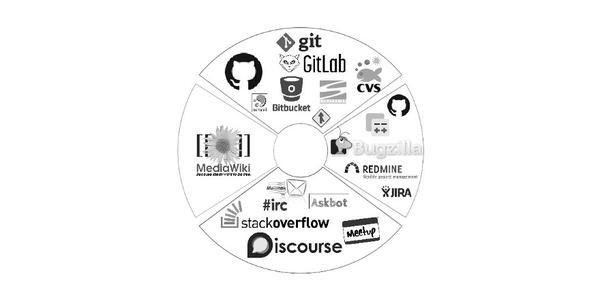
\includegraphics[width=90mm]{bitergia.jpg}
\caption{Bitergia data forums}
\end{figure}

Now that they had the tools ready to extract the data, the next step was to build a framework which would help them to analyze and then visualize the data which they would obtain from the MetricsGrimoire tools. This is known as the \emph{VizGrimoire Library} and has two important tools in it -

1.vizGrimoireR : After extracting the needed data, this tool helps in analyzing the dataset to produce data which then can be used to answer specific type of questions.

2.vizGrimoireJS : Having the right kind of data in hand led to the need to have a dashboard kind of environment to shocase the data in a meaningful way. This tool hence creates dashboards with reports and visualizations of the data.

\section{Task at hand}
We were presented with two cases which needed improvised visualizations. The existing visualizations were not feasible to answer different kinds of questions that one can pose. We had to work through various visualizations in order to finalize on a nearly good enough solution. We will first talk about each of the two cases presented to us and then discuss the solutions that we fixed upon in the next chapter.

 \textbf{CASE 1 -Where do Developers work ?}

Location has always been of importance in any area of work. In the software industry, distance always was not a matter of concern because of the nature of work involved, with this being even more true for Open Source Software as its developers are assumed to be contributing according to their convenience \cite{yuri2010}. Considering this, the group at Bitergia decided to investigate the overall spread of developers across the world for a few projects. Their main database was the data they collected from github and mailing lists for those organizations. There were certain assumptions involved like the timezones mentioned in the mail tools were correct and that they correspond to the geographical areas to some extent. They came up with these two basic visualizations as a start to analyzing the data.

\begin{figure}[!ht]
\centering
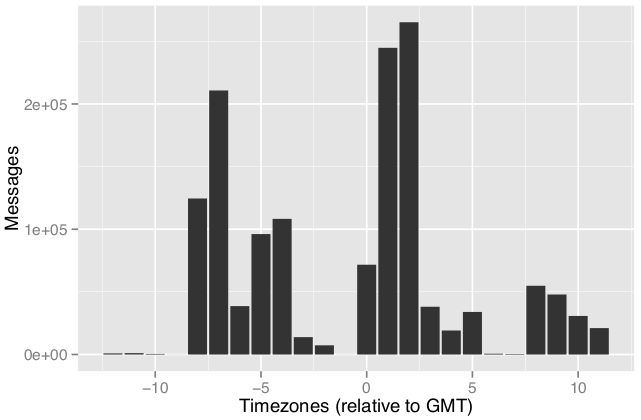
\includegraphics[width=90mm]{work1.png}
\caption{Timezone origin of messages}
\end{figure}

\begin{figure}[!ht]
\centering
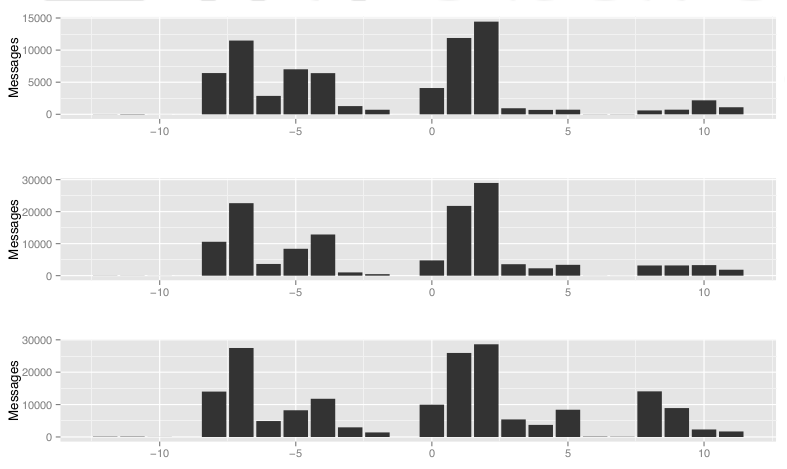
\includegraphics[width=90mm]{work2.png}
\caption{Timezone origin of messages for 2002,2007,2012}
\end{figure}

The following was the division of geography with respect to timezone -

1. America: GMT-8 to GMT-2 (US/Canada: -8 to -4)

2. Europe/Africa/Middle East: GMT to GMT+5

3. East Asia/Australia: GMT+8 to GMT+11


The visualizations being very basic didn't help solve or understand a lot about the developer spread for an organization. They were more oriented in giving an overview of messages per timezone. It was not clear about the relation between commits and authors and location tied together which needed more than a birds' eye view type of a visualization. 

\textbf{CASE 2 - Experience of Developers}
A lot has been discussed about the motivation for developers to join or stay or leave an open source project. The most sort after work being the onion model which describes the general roles that developers take and how they gravitate eventually \cite{crowston2005,  kishida2003}. The Bitergia team focused on calculating age in project for active developers at a certain time. They again had access to datasets which gave them the data needed to calculate the same. As a result of their work the following visualizations were built - 

\begin{figure}[!ht]
\centering
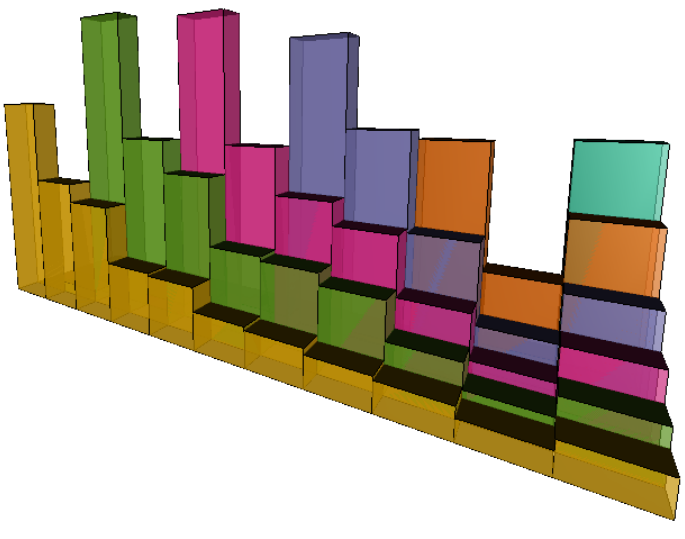
\includegraphics[width=90mm]{age2.png}
\caption{3D version of pyramids every two years}
\end{figure}

\begin{figure}[!ht]
\centering
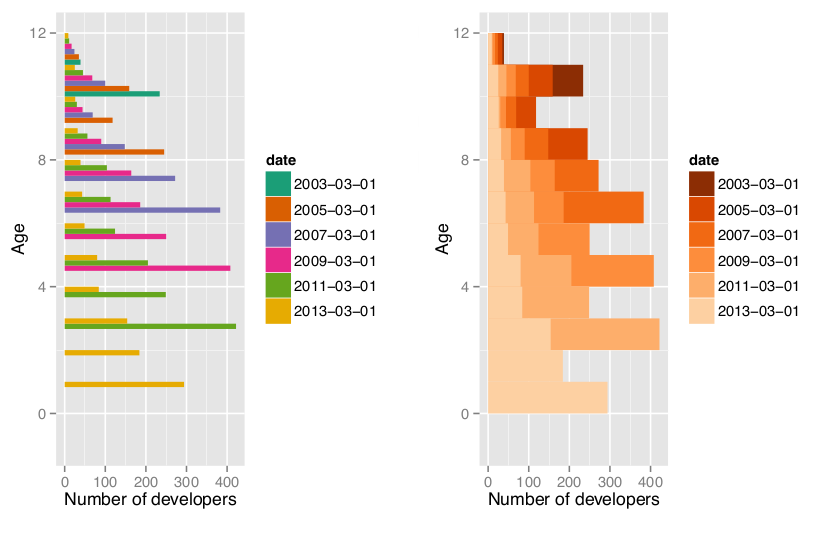
\includegraphics[width=90mm]{age1.png}
\caption{Comparison for pyramids every two years}
\end{figure}

The problem here was that, the 3D visualization, though colorful, was a little hard to relate to understand the dynamics. WHAT ELSE IS WRONG ?????? My visuals are the same!


\chapter{Methodology}
To help explore the previously explained cases, our task was to look into improvising the visualizations to help people understand the data in a better way. To carryout this process we took datasets of 5 open source projects for the cases explained in the previous chapter. We started off with different prototypes for each case and improvised by taking timely suggestions from the team. We build initial visualizations and followed an iterative process of development.  

\section{Dataset}
As Bitergia already had a large database for a few open source projects, they were very co-operative and gave us full access to all the data that they had in hand for the 5 organizations we were looking into. The files were all in the json format and this was an ideal format for us to work with as well. There was some manipulation of data involved for a few visualizations. The first step was to identify the format of the data and then brainstorm for ideal visualizations depending on the possible ways to understand the data. All the data collected was for February,2015 and has data from 2010 to 2015. The timezone files have data from timezone -12 to +11.One important field added to the timezone files, was the approximate population for each of the timezones which was taken from the below graph.

\begin{figure}[!ht]
\centering
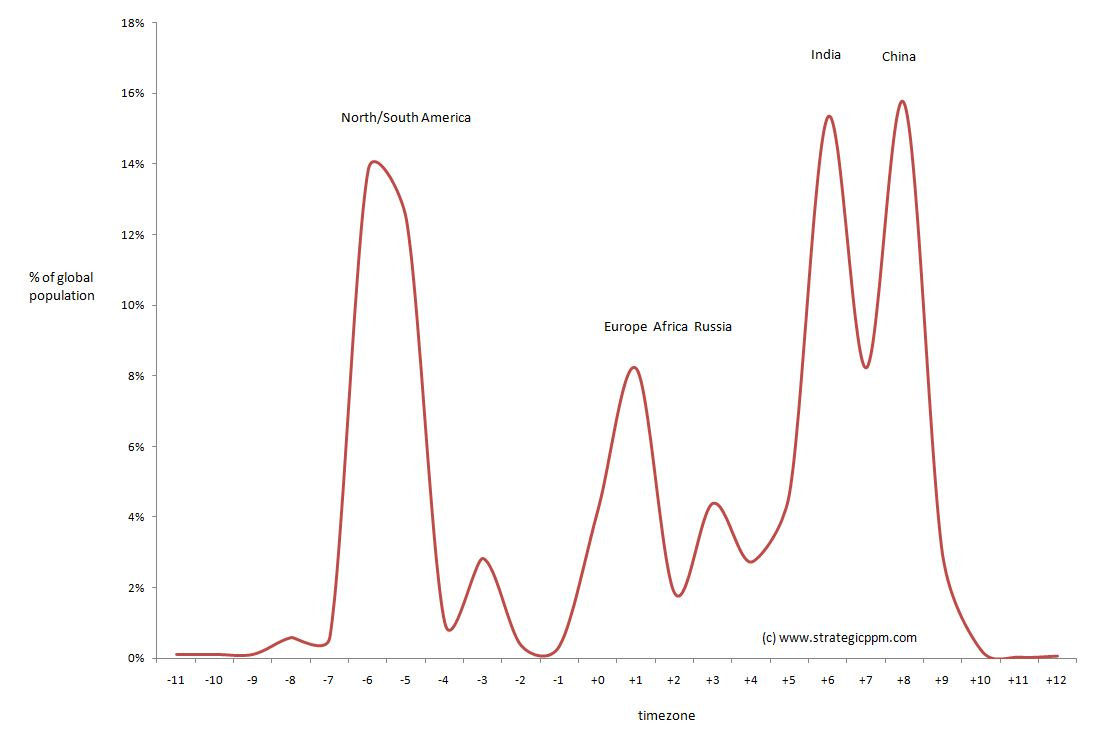
\includegraphics[width=90mm]{pop1.jpg}
\caption{Global population by timezone}
\end{figure}

Also in order to build a timezone based visualization, a geojson file was needed which would draw the map timezone wise and this file was found. As geojson files have large overhead and would take a lot of time to load, converting it to topojson format was better. Topojson is a command line application which not only reduces the size of geojson files, it also gives multiple options like simplification,conversion etc.It can be installed easily using NPM.

\section{The Organizations}

1. Eclipse Foundation :
This is a member supported open source community focused on building a platform comprised of extensible frameworks, tools and runtimes for building, deploying and managing softwares across the lifecycle.

2. OpenStack :
It is one of the most active open source products currently available for all types of cloud environments. It controls a a large number of resources for computation, storage ,networking for a datacenter.

3. Puppet Labs :
This is an open source tool which manages various stages of IT infrastructure inclusive of provisioning, patching, configuration and management of operating systems across cloud structures.

4. RedHat RDO:
This is a community of people who are interested to use and deploy OpenStack on the RedHat Linux, Fedora ditributions. It is a sub community of people who use RedHat which is one of the largest contributors to Linux.

5. Citrix Apache Cloudstack :
This is an open source software which deploys and manages networks of virtual machines as a IaaS(Infrastructure as a Service) platform. It supports VMware, KVM, XenServer, Hyper-V.




\section{D3.js}
As the visualizations needed flexibility the most ideal tool in hand was D3.js. D3 is a javascript library built by Mike Bostock which has the capacity to build interactive, dynamic and a big variety of visualizations. It is largely based on HTML5, CSS and SVG. It makes rendering the visualizations on any browser extremely convenient and easy as well. Due to the large developer support available for the library, it was an ideal choice to build the final visualizations in.It accepts external data in the form of json,CSV or TSV. Being a javascript library, it follows the same syntax hence making data manipulation quick. D3 API has hundreds of functions which make gives it its community. This library is widely used by big corporates like Datameer, The New York Times, OpenStreetMap etc.

\section{Initial Iterations}

\section{Final Implementations}

\begin{figure}[!ht]
\centering
\fbox{\huge Box}
\caption{Go figure.}
\end{figure}

\chapter{User study}
I have done some excellent research \cite{matrix}.
\section{Introduction to the Introduction}
\begin{figure}[!ht]
\centering
\fbox{\huge Box}
\caption{Go figure.}
\end{figure}

\chapter{Results}
I have done some excellent research \cite{matrix}.
\section{Introduction to the Introduction}
\begin{figure}[!ht]
\centering
\fbox{\huge Box}
\caption{Go figure.}
\end{figure}

\chapter{Conclusion}
Wow, that really was excellent.
\section{Fin}
This is the end, my only friend, the end.


\bibliographystyle{unsrt}
\bibliography{thesis}

\end{document}
